\documentclass[]{standalone}
\usepackage{tikz}
\usetikzlibrary{shapes,arrows,calc,positioning}
\usepackage{amsmath} % for dfrac

\tikzset{
    block/.style = {draw, rectangle,
        minimum height=1.2cm,
        minimum width=2cm},
    input/.style = {coordinate,node distance=1cm},
    output/.style = {coordinate,node distance=1cm},
    sum/.style = {draw, circle, node distance=1cm},
}

\begin{document}
        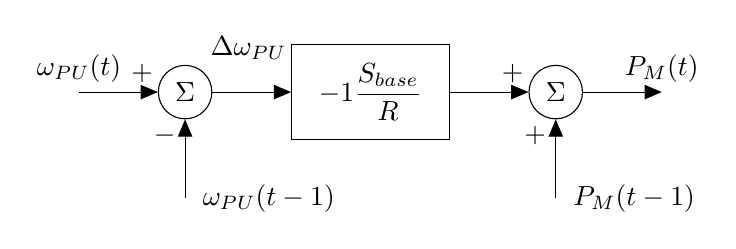
\begin{tikzpicture}[auto, node distance=1cm,>=triangle 45]
        \node [input, name=input, label=$\omega_{PU}(t)$] {};
        \node [sum, right=of input,label={55:$\Delta\omega_{PU}$}] (sum1) {$\Sigma$};
        \node [block, right=of sum1] (gain) {$-1 \dfrac{S_{base}}{R}$};
        \node [sum, right= of gain] (sum2) {$\Sigma$};
        \node [output, right=of sum2, label=$P_M(t)$] (output) {};
        
        \node [input, name=omega, below= of sum1,label={[label distance=.1cm]0:$\omega_{PU}(t-1)$} ] {};
       	\node [input, name=Pm0, below= of sum2,label={[label distance=.1cm]0:$P_{M}
       		(t-1)$} ]{};
       
        \draw [draw,->] (input) -- node[pos=0.8] {$+$} (sum1);
        \draw [->] (omega) -- node[pos=0.8] {$-$} (sum1);
        
        \draw [->] (sum1) -- (gain) ;
        \draw [->] (gain) -- node[pos=0.8] {$+$} (sum2);
        \draw [->] (Pm0) -- node[pos=0.8] {$+$} (sum2);
        \draw [->] (sum2) -- (output);
        
        \end{tikzpicture} 
\end{document}